\documentclass{article} %fleqn
\usepackage[english]{babel}
\usepackage[letterpaper,top=1cm,bottom=1cm,left=3cm,right=3cm,marginparwidth=1.75cm]{geometry}  %Template line
\usepackage{amsmath}
\usepackage{xcolor}
\usepackage{framed}
\usepackage{tikz}
\definecolor{brownie}{HTML}{FF822E}
\usepackage[colorlinks=true, allcolors=blue]{hyperref}
\title{\color{brownie}{My $\LaTeX$ Playground}}
\author{Rohan Thomas}

\begin{document}
\maketitle
\section{Introduction to Double Integrals}

The motivation of Double Integrals came from the notion of a "volume problem" which is to find the volume under a surface over a region. Similar to a single integral, the definition of a double integral is given as the limit of a Riemann Summation which is discussed below.  
\newline

\begin{framed}
\textbf{Definition:} If $f$ is a function of two variables that is
continuous and nonnegative on a region $R$ in the $xy$-plane, then the volume of the solid enclosed between the surface $z=f(x,y)$ and the region $R$ is defined by
\begin{equation}\label{reimann}
    V=\lim_{m,n\to\infty} \sum_{i=1}^m \sum_{j=1}^n f(x_k^*,y_k^*)\Delta A_k =\iint \limits_R f(x,y) dA 
\end{equation}
where $R$ is a given region.
\end{framed}

\section{Iterated integrals}
It's practically not possible to compute the volume every time using \eqref{reimann}, However, the Fundamental Theorem of Calculus helps us to compute it as an iterated integral.
\begin{equation*}
\int\limits_{a}^{b} \int \limits_{c}^{d} f(x,y) \,dx\,dy =\int\limits_{a}^{b} \underbrace{\left[\int \limits_{c}^{d} f(x,y) \,dx\right]}_{\text{fix y}}\,dy 
\end{equation*}

\subsection{Geometric Interpretation of an Iterated Integral; Volume by Slicing.}
Recall the definition of Volume of a solid. $V= \int \limits_a^b A(x) \,dx$ or $\int \limits_{c}^{d} A(y) \,dy$

\begin{center}
\tikzset{every picture/.style={line width=0.75pt}} %set default line width to 0.75pt        

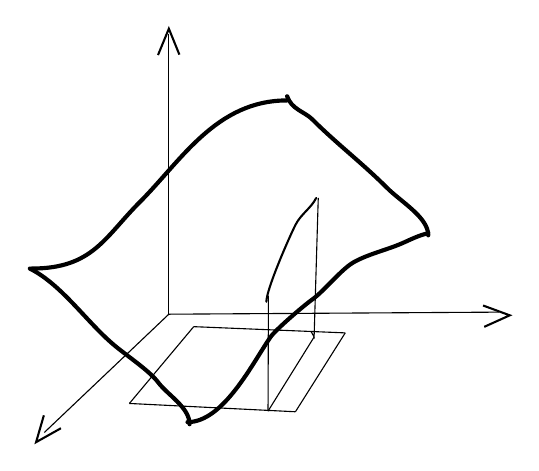
\begin{tikzpicture}[x=0.75pt,y=0.75pt,yscale=-1,xscale=1]
%uncomment if require: \path (0,300); %set diagram left start at 0, and has height of 300

%Straight Lines [id:da3235817911807528] 
\draw    (221.4,63.6) -- (221.4,198.6) ;
%Straight Lines [id:da49618028599845987] 
\draw    (221.4,198.6) -- (380.4,197.6) ;
%Straight Lines [id:da6884853742913688] 
\draw    (161.4,255.6) -- (221.4,198.6) ;
%Shape: Free Drawing [id:dp9815994491365303] 
\draw  [line width=1.5] [line join = round][line cap = round] (278.4,95.6) .. controls (244.27,95.6) and (227.47,124.53) .. (207.4,144.6) .. controls (190.54,161.46) and (184.71,176.6) .. (155.4,176.6) ;
%Shape: Free Drawing [id:dp3227544641358788] 
\draw  [line width=1.5] [line join = round][line cap = round] (346.4,159.6) .. controls (341.85,160.51) and (337.67,162.77) .. (333.4,164.6) .. controls (326.33,167.63) and (317.12,169.76) .. (310.4,173.6) .. controls (304.36,177.05) and (296.41,187.31) .. (290.4,191.6) .. controls (286.24,194.57) and (272.82,206.1) .. (270.4,209.6) .. controls (261.7,222.17) and (247.74,250.6) .. (230.4,250.6) ;
%Shape: Free Drawing [id:dp008422095874036417] 
\draw  [line width=1.5] [line join = round][line cap = round] (278.4,93.6) .. controls (280.5,99.89) and (286.88,101.08) .. (290.4,104.6) .. controls (302.13,116.33) and (314.63,125.83) .. (326.4,137.6) .. controls (333.34,144.54) and (346.4,151.94) .. (346.4,160.6) ;
%Shape: Free Drawing [id:dp1398603505639573] 
\draw  [line width=1.5] [line join = round][line cap = round] (154.4,176.6) .. controls (170.31,184.56) and (182.47,203.46) .. (196.4,214.6) .. controls (202.99,219.87) and (212.39,226.25) .. (216.4,231.6) .. controls (220.84,237.51) and (231.4,243.52) .. (231.4,251.6) ;
\draw  [line width=0.75]  (216.19,73.74) -- (221.42,61.05) -- (226.49,73.53) ;
\draw  [line width=0.75]  (372.79,194.4) -- (385.67,199.14) -- (373.39,204.68) ;
\draw  [line width=0.75]  (169.42,253.54) -- (157.45,260.25) -- (161.2,247.32) ;
%Straight Lines [id:da5256095289199105] 
\draw    (202.4,241.6) -- (282.4,245.6) ;
%Straight Lines [id:da3183943778989651] 
\draw    (282.4,245.6) -- (306.4,207.6) ;
%Straight Lines [id:da24753672919767045] 
\draw    (233.4,204.6) -- (306.4,207.6) ;
%Straight Lines [id:da2529077685860224] 
\draw    (202.4,241.6) -- (233.4,204.6) ;
%Straight Lines [id:da17524026229606093] 
\draw    (290,207) -- (291.4,209.6) -- (293.4,142.6) ;
%Straight Lines [id:da9504707936220944] 
\draw    (269.2,245.3) -- (269.4,189.6) ;
%Shape: Free Drawing [id:dp1570081134801784] 
\draw  [line width=0.75] [line join = round][line cap = round] (292.4,142.6) .. controls (289.93,147.54) and (285.01,150.37) .. (282.4,155.6) .. controls (278.98,162.44) and (268.4,186.75) .. (268.4,192.6) ;
%Straight Lines [id:da023869808961202166] 
\draw    (269.2,245.3) -- (291.4,209.6) ;

\end{tikzpicture}
\end{center}
\end{document}